\chapter{Geschichte}
\label{chap:geschichte}
Um die Frage zu beantworten, wie Docker die führende Container-Technologie wurde, wird im Folgenden die Geschichte dieser betrachtet. Dabei liegt der Schwerpunkt auf Lösungen und Probleme der Technologien.
 
\section{Container-Runtimes}
\label{sec:lxc2containerd}
Wie in \fref{tab:timelineContainers} zu sehen, sind Container keine neue Erfindung. Bereits 2008 wurde die erste volle Implementierung einer Container-Runtime mit LXC ver"-öffentlicht. Im folgenden Abschnitt wird ein Blick auf Container-Runtimes in der Vergangenheit geworfen und die Frage geklärt, wie Docker die erfolgreichste Runtime wurde.

\subsection{Vor LXC: Isolation mit Kernel-Patches}
\label{sec:geschichteVorLXC}

Bereits 1979 wurde mit \gls{acr-chroot} die erste, Möglichkeit der Isolation veröffentlicht. Diese kam mit dem Betriebssystem Unix V7 und erlaubte es erstmals, verschiedene Prozesse in unterschiedliche Dateisystemen zu trennen. Der Systemaufruf wurde 1982 in BSD hinzugefügt \citep{ABriefHistoryofContainers:fromthe1970sto2017}. 20 Jahre später rücken isolierbare Prozesse durch FreeBSD Jails in den Mittelpunkt. Diese erweitern das \Gls{acr-chroot}-Konzept, indem nicht nur das Dateisystem vom Host-System getrennt wird, sondern auch Hostnamen, IP-Adressen und die Nutzerverwaltung \citep{FreeBSDHandbook}. 

Neben FreeBSD Jails wurde bereits 2001 Linux VServer veröffentlicht, eine Software, die ähnlich wie Jails eine Isolation des Dateisystems und auch der Netzwerkadresse erlaubt. Entgegen der aktuell noch weiterentwickelten Jails war der letzte stabile Release von VServer 2008 \citep{PaperLinuxVServer}. Der größte Nachteil des VServers waren Kernel-Patches, die benötigt wurden, um die Isolierung zu gewährleisten.

In den folgenden Jahren wurden immer mehr Lösungen zur Isolation von Prozessen veröffentlicht, darunter Oracles Solaris Containers, das auf Zonen im Betriebssystem setzt und Open VZ, welches wie VServer, einen gepatchten Linux-Kernel benötigt, aber auch Ressourcen isolieren kann. Der größte Nachteil, denn alle diese Technologien haben, ist die unzureichende und komplizierte Virtualisierung einzelner Prozesse. Zudem müsssen Funktionen nachgepatched werden, die zur Isolation notwendig sind. Dies führte 2006 dazu, dass Entwickler von Google eine bessere Lösung entwickelten, Process Containers. Diese erlaubten ohne Patches eine einfache Verwendung und Isolation einzelner Ressourcen. Im Jahr 2007 wurden Process Container unter dem Namen \glspl{acr-cgroup} in den Linux-Kernel gemerged und liefern seitdem das Fundament für aktuelle Container-Technologien.

\subsection{LXC: Erste Schritte in Container-Runtimes}
\label{sec:geschichteLXC}
Mit \gls{acr-lxc} kam 2008 die erste vollwertige Implementation, die alleine mit dem nativen Kernel des Linux-\gls{acr-os} funktioniert (siehe \fref{tab:lxcKernel}). Damit löst LXC eins der größten Probleme der vorherigen Lösungen, indem kein gepachter Kernel benötigt wird.

\begin{table}[h]
		\begin{tabu} to \textwidth {@{}lX[2,l]@{}}
			\toprule
			Feature & Verwendung\\
			\midrule
			Namespaces & Trennung unterschiedlicher Systemkomponenten zur Virtualisierung\\
			Apparmor und SELinux & Mandatory Access Control\\
			Seccomp & Sicherheitsprofile, sperrt Systemaufrufe des isolierten Prozesses\\
			chroot und pivot\_root & Isolation des Dateisystems und Nutzernamespace-Mapping\\
			Capabilities & Entfernen von einzelnen Systemrechten\\
			CGroups & Verwalten der Systemressourcen\\
			\bottomrule
		\end{tabu}
	\caption{Von LXC genutze Kernel-Features \citep{Lxc7LinuxManualPage}}
	\label{tab:lxcKernel}
\end{table}

Ein weiterer Vorteil den \gls{acr-lxc} gegenüber älteren Technologien besitzt, ist die Einfachheit in der Benutzung. Im Gegensatz zu Linux VServern liefert \gls{acr-lxc} eine Konfigurationsdatei, vorgefertigte Seccomp oder SELinux Profile und ein \gls{acr-cli}. Diese erlauben es durch einfache Bash-Ko"-mman"-dos Container Prozesse in Containern zu isolieren. Dieser Vorteil ist allerdings auch ein großer Nachteil an \gls{acr-lxc}. \gls{acr-lxc} ist sehr systemnah und lässt sich durch die verwendeten Kernel-Features nur auf Linux-Systemen nutzen. Zudem ist die Konfiguration eines Containers weitreichender und komplexer als bei aktuellen Container-Runtimes.

\subsection{CF Warden: Innovation durch Vereinfachung}
\label{sec:geschichteCFWarden}
2011 wurde die erste kommerziellen Container-Runtime mit \gls{acr-cf} Warden veröffentlicht. Diese basierte zu Beginn auf \gls{acr-lxc} und erweiterte diese mit eigenen Funktionen, wie einer REST API zur Steuerung und Verwaltung eines Container Clusters. Dabei setzt \gls{acr-cf} Warden auf eine Client-Server-Architektur (siehe \fref{fig:wardenArch}). 

\begin{figure}[h]
	\begin{center}
		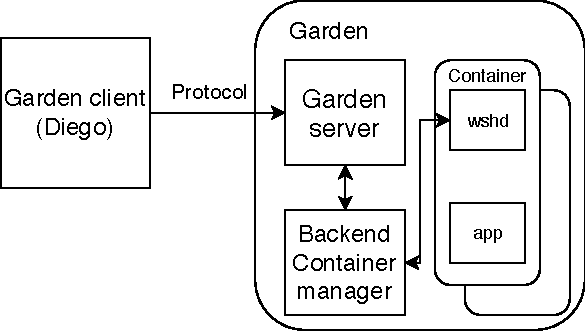
\includegraphics{bilder/cf-warden-arch.pdf}
		\caption{Client-Server-Architektur von CF Warden \citep{CFGardenbackEndsContainerSecurityDebugging}}
		\label{fig:wardenArch}
	\end{center}
\end{figure}

Im Gegensatz zu \gls{acr-lxc} ist \gls{acr-cf} Warden nicht mehr an Linux gebunden, sondern entkoppelt. Durch die Verwendung einer Bibliothek ist es möglich, Warden auch unter Windows Systemen zu verwenden. Warden kann als Container-Runtime für \gls{acr-cf}-Cluster genutzt werden, ist dort allerdings durch Garden ersetzt worden, einer Neuimplementation in der Sprache Go.

\subsection{\gls{acr-lmctfy} und Go: Googles Einfluss auf Container}
\label{sec:geschichteLMCTFY}
\gls{acr-cf} Warden wird nahezu ausschließlich innerhalb eines \gls{acr-cf}-Clusters genutzt. Eine lokale Nutzung ist dabei nicht der Schwerpunkt. Für den Entwicklungsprozess und für die Nutzung außerhalb einer \gls{acr-cf} Umgebung hat Google 2013 \gls{acr-lmctfy} veröffentlicht. Dieser Service bildet Googles Container-Stack ab. \gls{acr-lmctfy} wird nicht aktiv weiterentwickelt, die Kernkonzepte wurden allerdings in libcontainer übernommen und von Docker weiter entwickelt.

Eine weitere wichtige Entwicklung von Google, neben \glspl{acr-cgroup} und \gls{acr-lmctfy}, ist die Sprache Go. Diese findet in allen modernen Container-Runtimes Verwendung und ist eine der wichtigsten Entwicklungen der letzten 10 Jahre für Container. Dabei sind die Geschwindigkeit und Flexibilität von Go die wichtigsten Aspekte. Kompilierte Go-Programme laufen auf nahezu allen Systemen. Dabei sind die ausführbaren Binaries durch statisches Binden unabhängig von installierten Bibliotheken auf dem System. Zudem ist Go performanter als andere Sprachen.

\subsection{Docker: Ecosystem, Runtime und \gls{acr-saas} in einem}
\label{sec:geschichteDocker}
Im Jahr 2013 kam der größte Durchbruch für die Container-Technologie. Mit dem Release der Software Docker explodierten Container in Popularität und Nutzung. Wie auch \gls{acr-cf} Warden setzte Docker zu Beginn auf \gls{acr-lxc}. Der größte Unterschied zu bestehenden Container-Runtimes ist aber das Angebot als Ecosystem. Docker erlaubt es, \glspl{gls-image} aus dem Internet zu nutzen und bietet mit Docker Hub eine Plattform, die es sehr einfach ermöglicht, neue \gls{acr-saas}-Angebote für Kunden zugänglich zu machen. Zudem bietet Docker eine deutlich vereinfachte Form der Konfiguration mit Dockerfiles an. Durch die einfache Nutzung mittels \gls{acr-cli} und der Möglichkeit, seine Services als \gls{gls-image} bereitzustellen gelang es Docker, unangefochten die meistgenutzte Container-Software zu werden.

\section{Weiterführende Technologien}
\label{sec:timeline}
Anhand der Geschichte der Container-Technologien erkennt man, das die heutige Innovation auf dem Gebiet der Isolation und Virtualisierung stark durch Container angetrieben wird. Vor allem Docker und Google, aber auch Microsoft oder Amazon treiben die Technologie an. Dabei wird immer ein Fokus auf die einfachere Nutzung gelegt, sowie die Automatisierbarkeit einzelner Prozesse, wie dem Bereitstellen oder kompilieren einer Anwendung.

\fref{tab:timelineContainers} gibt einen Rückblick auf die Geschichte der Container-Technologie. Dabei wird der zeitliche Hergang einzelner Funktionen und Runtimes in Bezug gestellt und aktuelle Themen aufgezeigt.
\begin{table}[h]
	\providecommand{\timeline}{\color{LightSteelBlue3}\makebox[0pt]{\textbullet}\hskip-0.5pt\vrule width 1pt\hspace{\labelsep}}
	\renewcommand{\arraystretch}{1}
	\begin{center}
		\begin{tabu}to 0.9\textwidth{@{}r <{\hskip 3pt} !{\timeline} X[2,l]@{}}
			\toprule
			      \multicolumn{2}{c}{\textbf{Benötigte Technologien}}       \\ \midrule
			1979 & Unix V7 mit chroot                                       \\
			1998 & SELinux                                                  \\
			     & AppArmor                                                 \\
			1999 & Linux Capabilites                                        \\
			2000 & FreeBSD Jails                                            \\
			2001 & Linux VServer                                            \\
			2002 & Linux namespaces                                         \\
			2004 & Solaris Container                                        \\
			2005 & Open VZ                                                  \\
			2006 & Google Process Container                                 \\
			2007 & Process Container in Linux Kernel als \glspl{acr-cgroup} \\
			2012 & Erste stabile Version der Sprache Go                     \\ \midrule
			        \multicolumn{2}{c}{\textbf{Container-Runtimes}}         \\ \midrule
			2008 & \gls{acr-lxc}                                            \\
			2011 & \gls{acr-cf} Warden                                      \\
			2013 & \gls{acr-lmctfy}                                         \\
			     & \gls{acr-cf} Graden, Umstieg auf Go                      \\
			2014 & \Gls{acr-appc} Spezifikation Release                     \\
			     & Release rkt                                              \\
			2015 & Release LXD                                              \\
			     & Release runC                                             \\
			2016 & Windows Containers                                       \\
			     & \gls{acr-cf} Guardian Release, Support für runC          \\
			2017 & Release containerd v1.0.0                                \\
			     & Release cri-o                                            \\ \midrule
			 \multicolumn{2}{c}{\textbf{Entwicklung Container-Ecosystem}}   \\ \midrule
			2011 & Initialer Release \gls{acr-cf}                           \\
			2013 & Release Docker, erstes Container Ecosystem               \\
			2014 & Entwicklung \gls{acr-k8} startet                         \\
			2015 & Gründung \gls{acr-cncf} und \gls{acr-oci}                \\
			     & Docker Swarm                                             \\
			2016 & "Dirty Cow" $\rightarrow$ Container Sicherheit           \\
			     & Apache Mesos v1.0.0 Release                              \\
			2017 & Übernahme rkt und containerd in \gls{acr-cncf}           \\
			     & Release \gls{acr-oci} runtime-spec und image-spec        \\ \bottomrule
		\end{tabu}
		\caption{Timeline Container-Technologien \citep{ABriefHistoryofContainers:fromthe1970sto2017}}
		\label{tab:timelineContainers}
	\end{center}
\end{table}
